\chapter{G. Ramachandran – A great mind, a great soul}

\Authorline{Srinivasan Anand}
\medskip


G. Ramachandran, GR, teacher par excellence and a great thinker has always been and will continue to be an inspiration to me. I consider myself blessed to have him as my teacher and mentor. It was a string of fortunate coincidences that brought me in contact with him in 1983. I was in the third year of my bachelors when I first met him. I had derived some equations relating to special theory of relativity but did not know how to take it further. My teachers in the college recommended that I contact GR.  I still recall vividly the sunny afternoon when I went to his office, nervous and anxious.  When I walked in he was staring at the black board full of equations, his right hand near his chin holding a chalk piece and his left hand behind his back holding his trouser belt. He turned and with a smile asked what I wanted. As if by magic, all my inhibitions disappeared, and I eagerly took out the sheets of paper with my so-called derivations. He took a quick glance. Then gave me a chalk piece and asked me to work it out on the black board.  All the time, he was asking questions steering me in specific directions which became apparent to me only much later when he showed me a book on special theory of relativity. Subsequently, whenever I had free time, I used to go to meet him either at the department or at his house. These interactions with him were decisive in inspiring me to pursue M.Sc.\ physics at the University of Mysore, and later on, an academic career in spite of all the struggles and uncertainties. 

During the two years of my M.Sc., I had the privilege of having many more “black-board” sessions where GR by his gentle nudges and questions brought out the physics right then and there. GR had a rare talent and insight to get the best out of his students.  His classes were dynamic – the way he taught made sure we were involved and interacting. When we were not fully prepared, which was often, he adjusted his lectures – but left us with a conscious drive to work harder for the next lecture. Characteristic features of his lectures were the spontaneity and flow – everything fell in place and concepts evolved fluidly. He also taught us how to cross-check results and get back on mistakes by tracing back to first principles. He mentored me even during my Ph.D.\ days and supported me during difficult phases in the early stages of my Ph.D.

Physics was not the only Ph.D.\ thing he taught me. Our discussions also touched upon religion, philosophy, ethics in science and life. Quite often, in the evenings I used to accompany him on his way home and sometimes linger at his home discussing. Not once can I recall him discouraging me or being irritated. He seemed to have infinite patience. Now in retrospect, I feel how over-bearing I must have been. Dear GR, it is all your selfless efforts – conscious and unconscious – that continue to help me in my research and teaching and mentoring my students.
\bigskip

\centerline{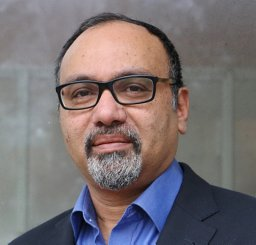
\includegraphics[scale=0.5]{figures/authors/Prof_Srinivasan_Anand.jpg}}
\smallskip

\authbio{Srinivasan Anand}
\bigskip

\noindent
\textbf{Dr.~Srinivasan Anand} obtained the M.Sc. degree in 1986 from Mysore University and Ph.D. in 1993 from TIFR, Mumbai. He worked as a Postdoctoral Fellow at the Department of Solid State Physics, Lund University, Sweden, from 1993 to 1997. He joined the Department of Applied Physics, School of Engineering Sciences, KTH --- Royal Institute of Technology, Sweden, where he is currently a Professor.
